
\chapter{Diseño de la unidad tractora de filamento}
\label{ane:tractora}
El material del que dispondremos será el siguiente.

\begin{itemize}
	\item{\textbf{Arduino Mega:} Microcontrolador encargado de mover un motor y regular su velocidad.}
	\item{\textbf{RAMPS:} Placa auxiliar colocada encima del arduino Mega, la cual dispone de un driver A4988 para controlar varios motores paso a paso.}
	\item{\textbf{Motor paso a paso:} Dispositivo electromagnético, que transforma una serie de impuslos eléctricos en desplazamientos angulares.}
\end{itemize}

Se vuelve a elegir un motor paso a paso como unidad de tracción, debido a las mismas razones por las que se eligió en la peletizadora.\\

El principio de funcionamiento de un motor paso a paso es sencillo. En el interior del mismo se dispone de dos bobinas giradas $90^oc$ entre sí \cite{pasoapaso} las cuales, en función de una secuencia de excitación, generarán campos magnéticos que hará que el rotor del mismo giré un determinado ángulo. Para la realización de la tractora, se usará una ténica denominada de micropasos con la que conseguimos que nuestro motor de $1.8 \circ$ de giro pueda alcanzazr grados de $0.225^o$. Para poder controlar el motor con está técnica y conseguir una velocidad de rotación constante, será necesario que el microcontrolador genera una señal cuadrada, en la que dependiendo de la frecuencia de esta señal, el motor girará a una velocidad distinta. El nivel alto de esta señal cuadrada, se la denominará paso. Por cada paso que reciba el motor, girará $1.8^o $ dividido el número de micropasos configurados en el driver:

\begin{table}[H]
    \centering
    \begin{tabular}{cccc}
        {\bf MS1} & {\bf MS2} & {\bf MS3} & {\bf Resolución de micropaso}  \\
        \hline
        L         & L         & L         & Paso completo (1)              \\
        H         & L         & L         & Medio paso (1/2)               \\
        L         & H         & L         & Un cuarto de paso (1/4)        \\
        H         & H         & L         & Un octavo de paso (1/8)        \\
        H         & H         & H         & Un dieciseisavo de paso (1/16)
    \end{tabular}
    \caption{Resolución del driver en función del micropaso elegido}
    \label{tab:res_drive}
\end{table}

Para el caso que nos ocupa, elegiremos la configuración de un dieciseisavo de resolución,es decir:

$$ \text{Pasos por vuelta} = \frac{360^o}{1.8^o \cdot \frac{1}{16} } = 3200 \text{pasos}  $$

Por tanto, si quisieramos girar el motor a una velocidad de $1RPM$ tendríamos que da un total de:

$$\frac{1 RPM \cdot 3200 pasos}{60 s} = 53 pasos/s$$

O lo que es lo mismo, un paso cada $18.86 ms$. Esta separación temporal, va inversamente relacionada con la velocidad de giro deseada, cuanta más velocidad de giro queramos, menor será el tiempo entre pasos. Para poder generar el tren de pulsos, se usará una interrupción del mirocontrolador, que se ejecutará cada $10\mu s$ e irá incrementando un contador, el cual, al llegar a un valor máximo determinado por la velocidad de giro, efectuará un escalón. El valor máximo del contador viene dado por la fórmula:

$$ Valor_{Max} = \frac{\text{Separación temporal de ticks}}{\text{Tiempo de interrupción}}$$

En nuestro caso, para girar el motor a una velocidad de 1RPM con una interrupción de $10\mu s$ deberíamos contar el siguiente número:

$$Valor_{Max} = \frac{18.75 ms}{10\mu s} = 1875$$

Por especificación del filastruder, determinamos que la velocidad de tracción deberá ir entre el rango de 1RPM y 3RPM, por tanto, con ayuda de una hoja de cálculo de excel, determinamos los valores máximosa a contar en función de la velocidad de giro.

\begin{table}[H]
    \centering
    \begin{tabular}{cccc}
        \multicolumn{1}{l}{{\bf RPM}} & \multicolumn{1}{l}{{\bf TICKS/S}} & \multicolumn{1}{l}{{\bf Separacion ticks (s)}} & \multicolumn{1}{l}{{\bf Ticks a contar por ISR}} \\
        \hline
        0 & -1 & -1 & -1 \\
        1 & 53 & 0,01875 & 1875 \\
        2 & 107 & 0,009375 & 938 \\
        3 & 160 & 0,00625 & 625
    \end{tabular}
    \caption{Valores para controla la velocidad de giro del motor paso a paso}
    \label{tab:valores_paso_paso}
\end{table}

Por tanto, cuando el contador llegue a los valores máximos establecidos, se generará un pulso, haciendo que el motor avance los grados determinados. A su vez, la velocidad de giro, vendrá dada por el PLC el cual, en función de un tensión de 0 a 5 V hará que el motor giré a una velocidad distinta.\\

Una vez establecida la arquitectura del software, se pasa a diseñar las piezas necesarias para crear la unidad tractora. Como la vez anterior, usaremos la herramienta Autodesk Inventor. Como unidad tractora, se diseñará una pieza que irá acoplado al eje de giro del motor, la cual irá recubierta por una goma para aumentar la fricción con el filamento. Con ayuda de un rodamiento haciendo presión por la otra parte del filamento, conseguiremos que se desplace de forma lineal

\begin{figure}[H]
    \centering
    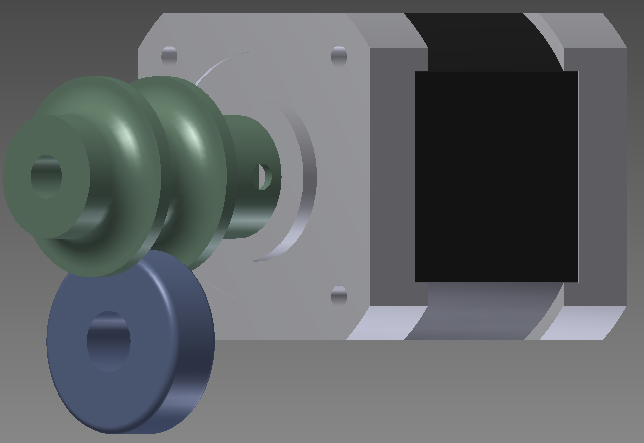
\includegraphics[width=0.6\textwidth]{images/producciones/tractora/motor.png}
    \caption{Diseño del eje de giro de la tractora}
    \label{fig:tractora}
\end{figure}


La pieza que soporte el rodamiento, deberá ir apretada por un muelle, para conseguir que asuma los cambios de diámetro y pueda hacer desplazar cualquier filamento sin importar el diámetro.

\begin{figure}[H]
    \centering
    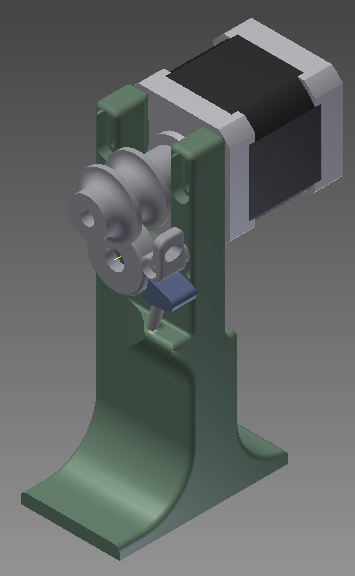
\includegraphics[width=0.5\textwidth]{images/producciones/tractora/asembli.png}
    \caption{Diseño de la tractora}
    \label{fig:tractora2}
\end{figure}

Una vez diseñadas las piezas, se pasan a imprimir en una impresora 3D

\begin{figure}[H]
    \centering
    \begin{subfigure}[b]{0.3\textwidth}
        \centering
        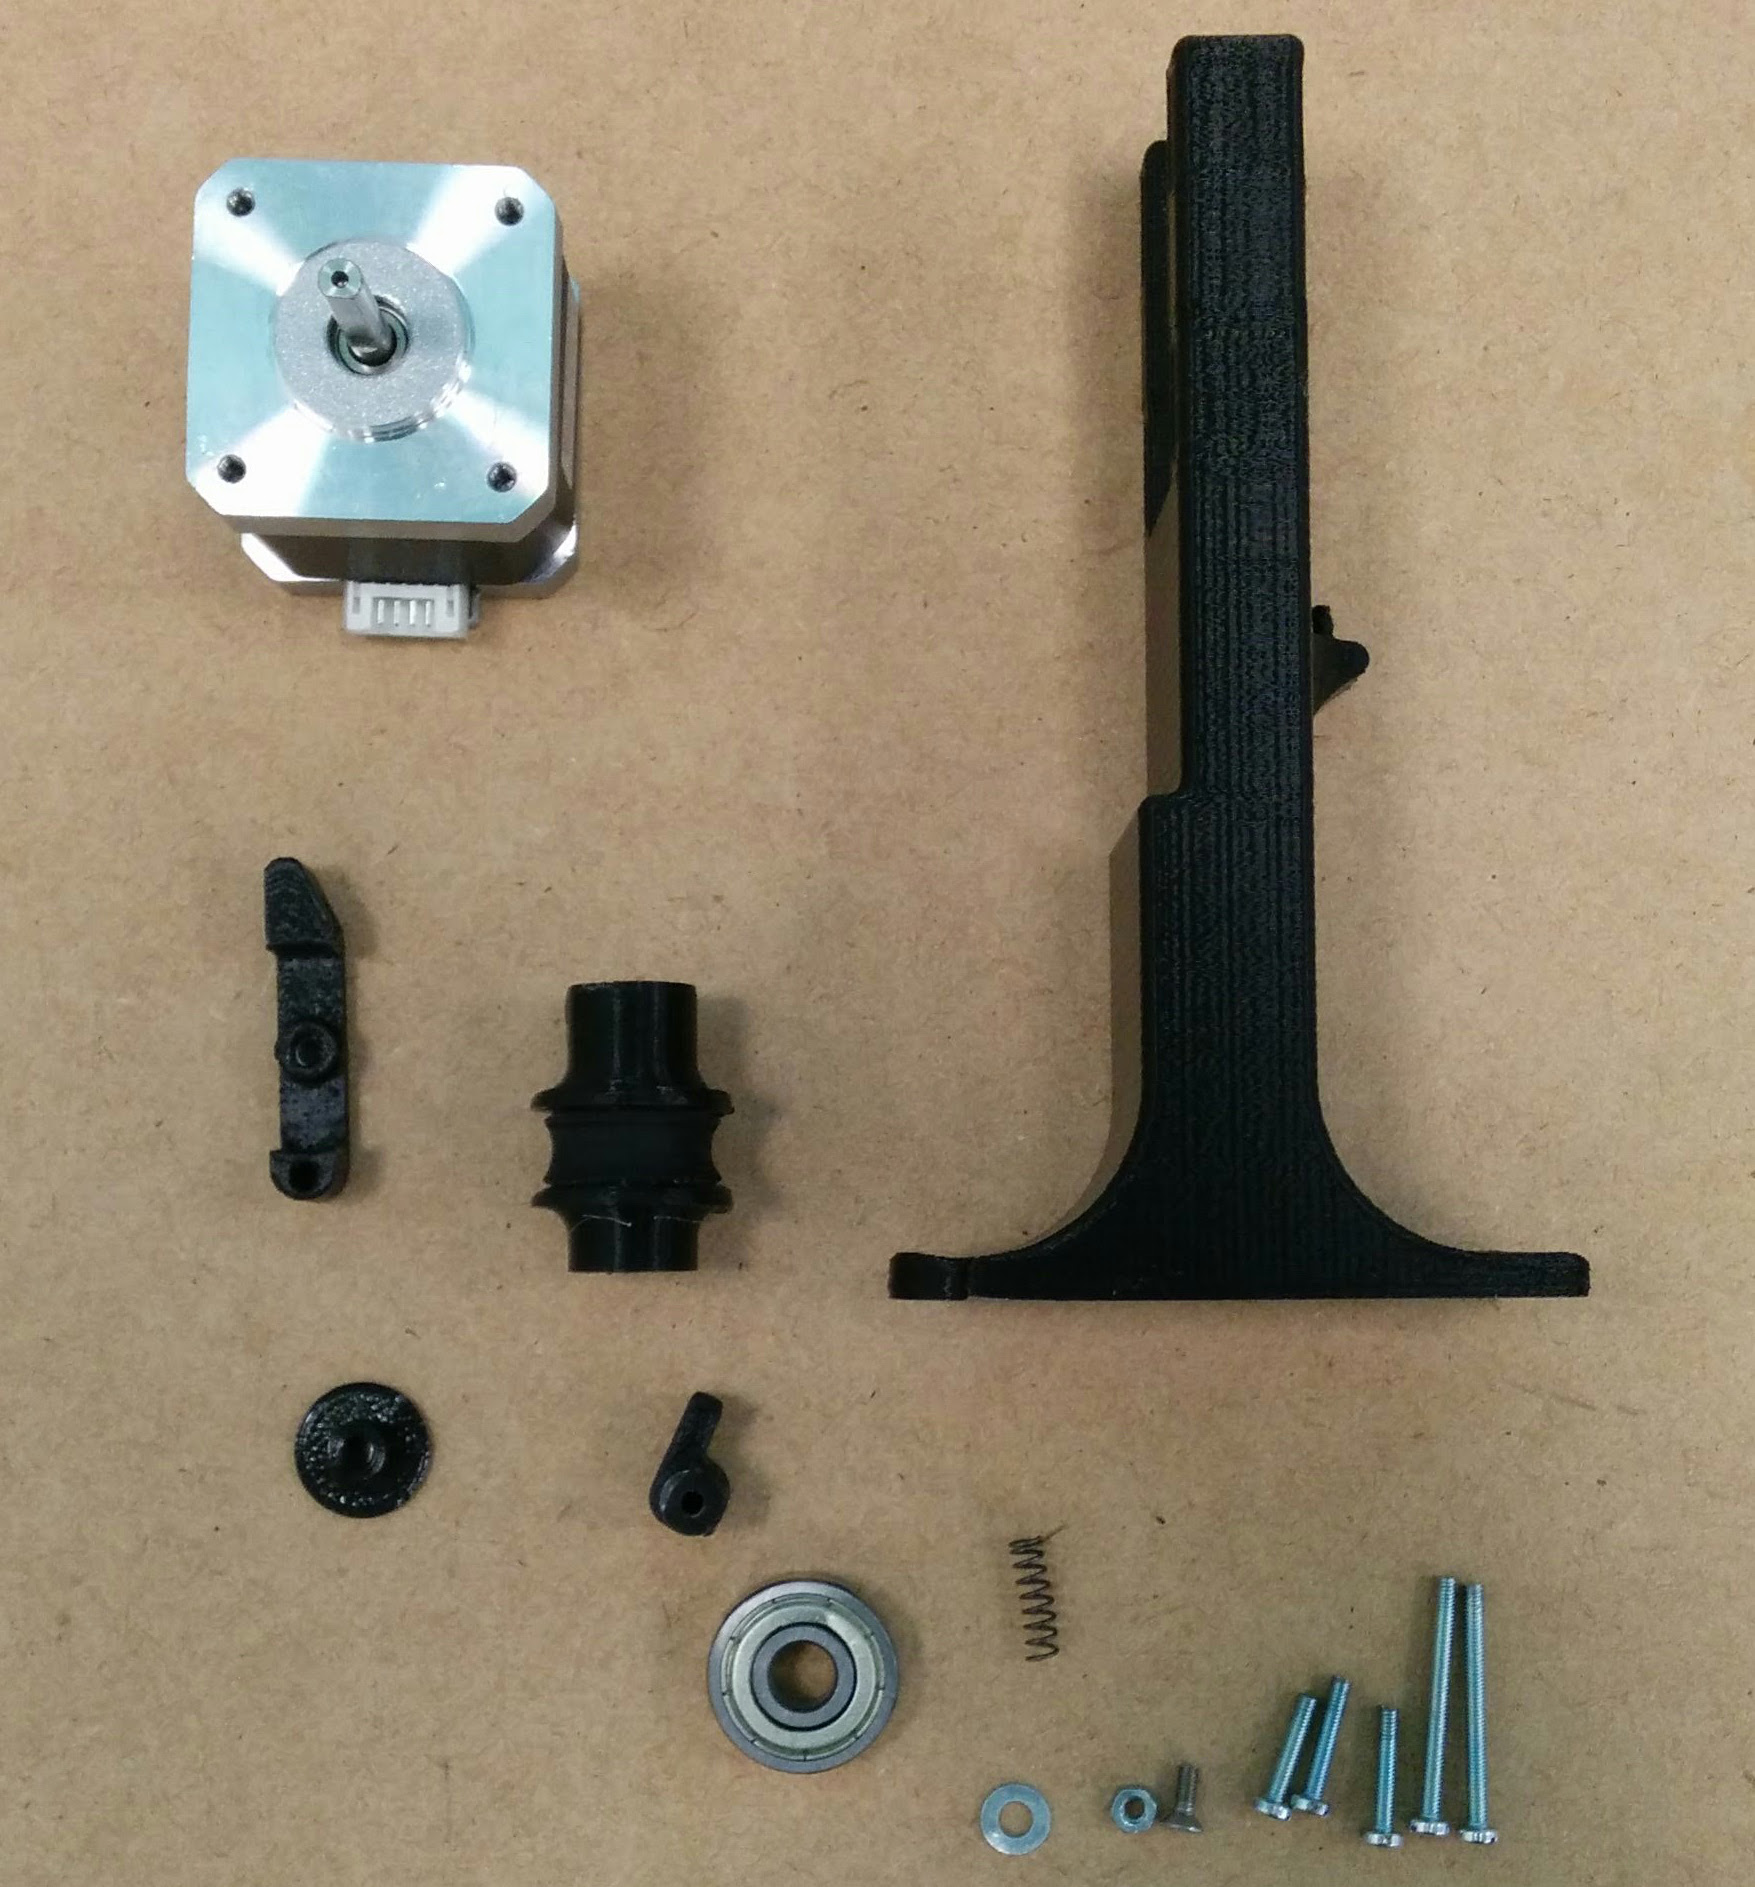
\includegraphics[width=\linewidth]{images/producciones/tractora/IMG_20150804_085937.jpg}
        \caption{Piezas impresoras de la tractora}
        \label{fig:tractora_piezas}
    \end{subfigure}
    ~
    \begin{subfigure}[b]{0.3\textwidth}
            \centering
        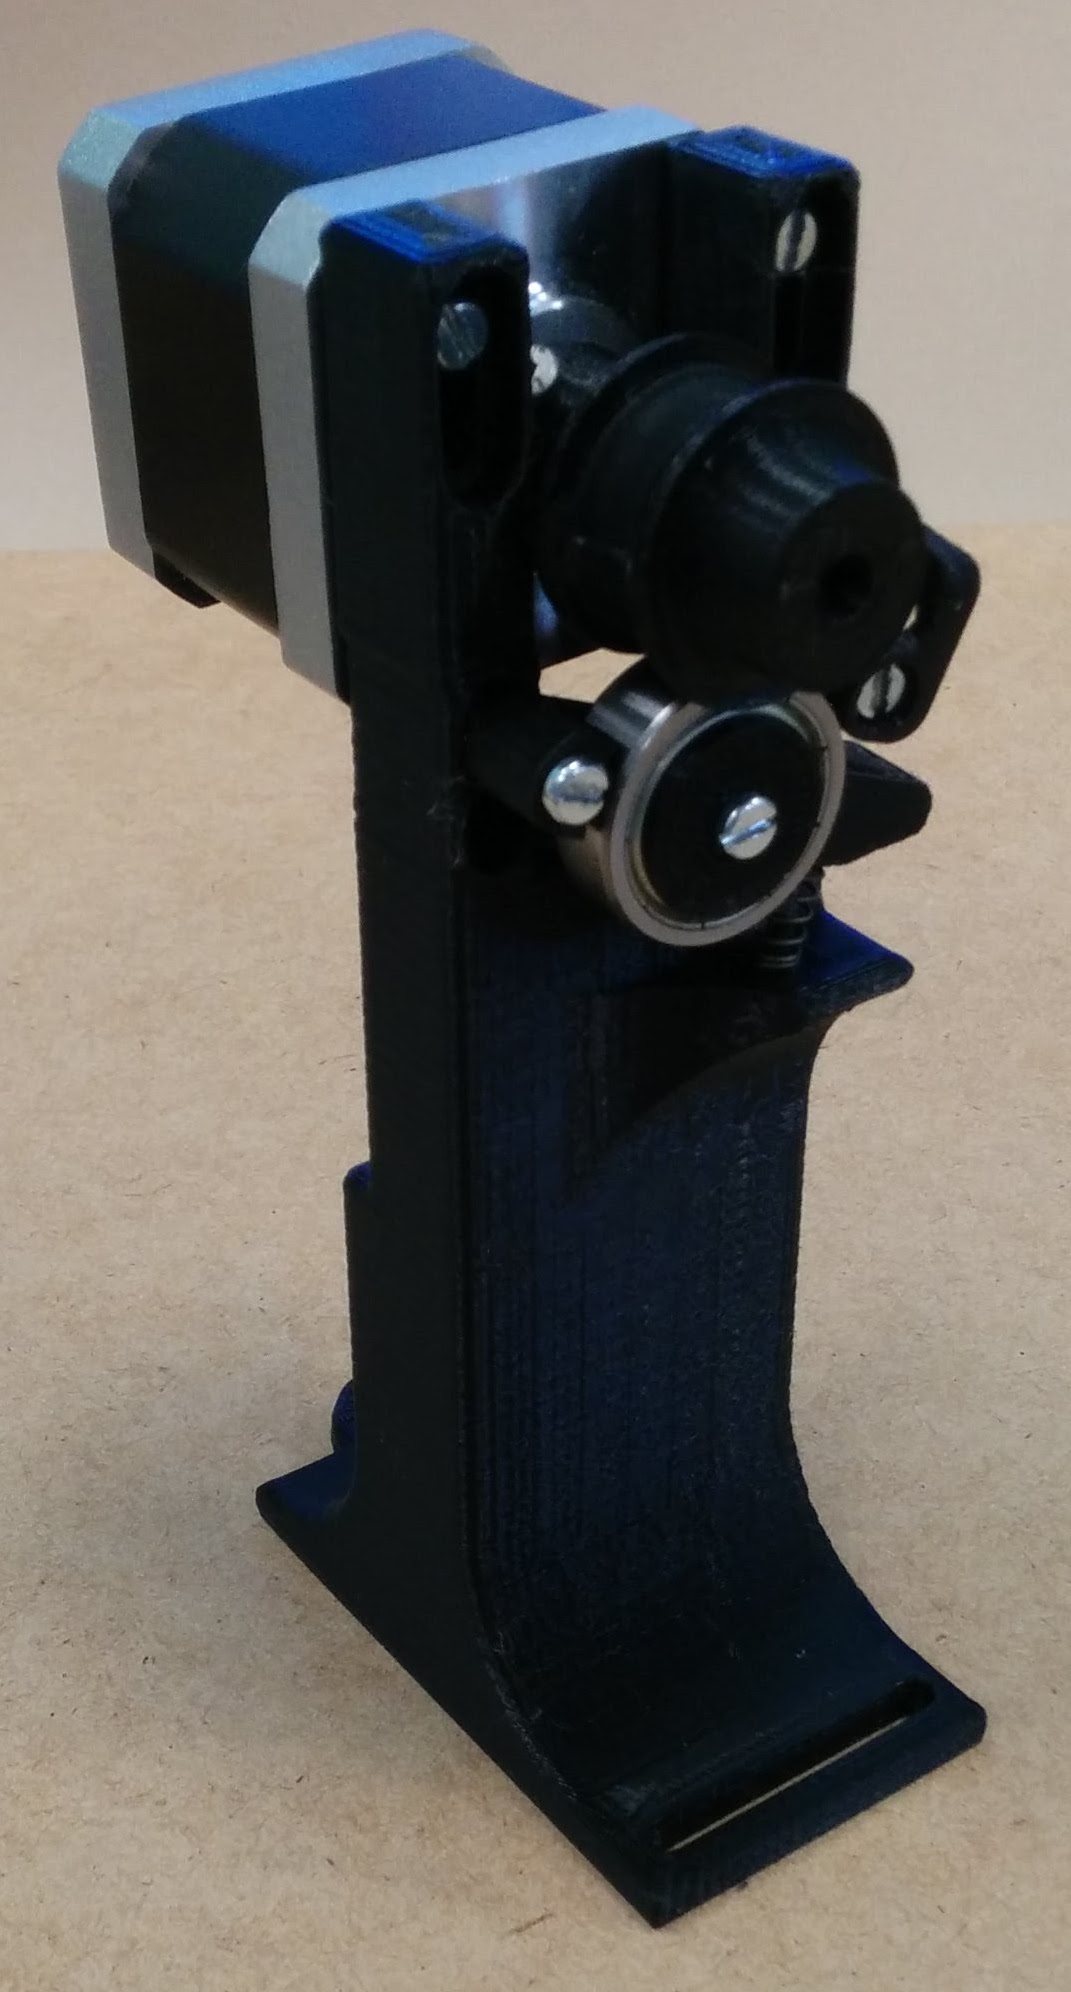
\includegraphics[width=\linewidth]{images/producciones/tractora/IMG_20150804_090625.jpg}
        \caption{Tractora montada}
        \label{fig:tractora_montada}
    \end{subfigure}
    \caption{Pieza de la tractora.}
    \label{fig:tractora_montaj}
\end{figure}

Por último, para comprobar que el funcionamiento de la tractora es el esperado, se hace pasar una bobina de filamento através de la tractora, y comprobamos que podemos variar la velocidad de tracción y el agarre del filamento es el adecuado.

	\begin{figure}[H]
            \centering
            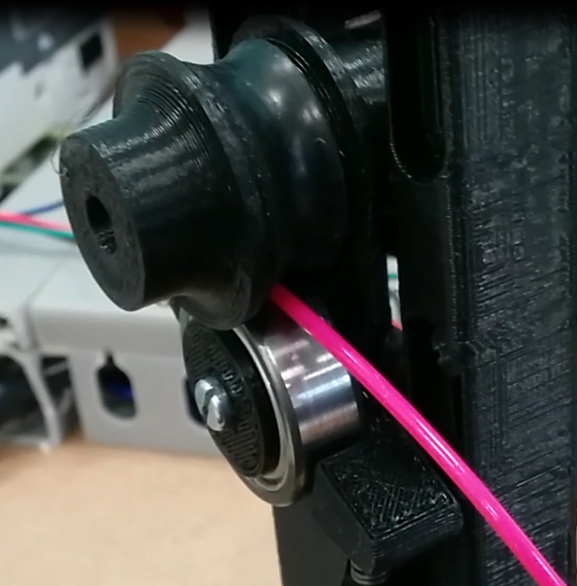
\includegraphics[width=0.5\textwidth]{images/producciones/tractora/final.png}
            \caption{Tractora con filamento}
            \label{fig:tractora_fila}
    \end{figure}
